\documentclass[12pt]{article}

\usepackage[a4paper,top=2cm,bottom=2cm,left=2cm,right=2cm,marginparwidth=1.75cm]{geometry}

% Useful packages
\usepackage[affil-it]{authblk}
\usepackage{algorithm}
\usepackage{algpseudocode}
\usepackage{amsmath}
\usepackage{graphicx}
\usepackage[colorlinks=true, allcolors=blue]{hyperref}
\usepackage[
        backend=biber,
        style=authoryear,
        sorting=nyt,
    ]{biblatex}
\addbibresource{ref.bib} 
\usepackage{epigraph} % for quoting
\usepackage{float}
\usepackage{amsfonts}
\usepackage{caption}
\usepackage{array} % Required for using p{width} column type

\title{As a Coin Side of Development:\\ Inequality Unconditionally Caused by Technology}

%\author[1,+]{Khanh Duong}
\author{}
%\affil[1]{\small UNU-MERIT, Maastricht, The Netherlands}
%\affil[+]{\small Corresponding author: duong@merit.unu.edu}


\date{} % This line hides the date

\begin{document}
\maketitle

\section{Introduction}

We often talk about economic development, but do we truly understand it? Although development can be defined differently from various perspectives, it is clear that it cannot be reduced to economic growth as measured by GDP per capita. Development can also be understood in non-monetary terms, such as well-being or happiness \parencite{agrawal2024economic}. However, do we agree that Bhutan, one of the happiest countries in the world, is more developed than the United States? Or that hunter-gatherer societies, often described by \textcite{sahlins2013original} as among the most affluent societies, are more developed than contemporary ones? Development, in this case, represents a choice between growth and equality, as inequality helps explain the paradox between growth and happiness \parencite{oishi2015income}. Although there are trade-offs between growth and equality \parencite{okun2010equality}, as well as between monetary and non-monetary aspects of development \parencite{kahneman2010high}, the former often determines the latter. For instance, humanity has historically moved away from an equal but impoverished existence in primitive societies to a wealthier, yet deeply unequal one. This progression aligns with the view that the United States is considered more developed than Bhutan, reflecting the dialectical notion that material conditions shape consciousness \parencite{lefebvre2009dialectical}.

Here, I will not delve too deeply into the broader definitions of development but will instead focus on monetary development, as it plays a decisive role. However, I do not limit monetary development to a narrow measure like GDP per capita. Imagine development as a wealth (or income) distribution: GDP per capita represents its first moment (the mean value), while the inequality corresponds to its second moment (the variance). I may not need to explore the highest moments, as inequality is sufficient to be considered a root cause of major social problems \parencite{neckerman2007inequality}, including climate change \parencite{duong2023does} and the socio-economic consequences of the pandemic \parencite{stantcheva2022inequalities}. If we simplify development into a coin, growth and inequality are its two sides \parencite{berg2017inequality}. One might argue that my statement assumes a trade-off between growth and inequality \parencite{okun2010equality}, which remains a contested issue. For instance, the Kuznets curve suggests that beyond a certain threshold, growth and equality can coexist \parencite{nielsen1997kuznets}. Similarly, the concept of sustainable development advocates growth accompanied by reduced inequality \parencite{freistein2016potential}. This discussion is also related to the debate on whether inequality is a matter of choice \parencite{stiglitz2013inequality}. Namibia, for example, is often cited as a country that has successfully reduced inequality through deliberate policy interventions \parencite{lawson2017inequality}, providing a counterexample to the inevitability of inequality in the development process.

Through this research, I provide evidence supporting the argument that if development (growth and inequality) is a choice, then they coexist, implying a trade-off between growth and equality (see Section \ref{sec:inequality}). Some may fear that this trade-off would inevitably lead to extreme inequality, which could hinder future growth \parencite{berg2017inequality} -an outcome that seems counterintuitive. However, my findings demonstrate that the trade-off occurs with a controlled inequality (a Gini index of less than 30). The evidence I provide is based on multi-objective optimisation, assuming that inequality and growth are choices within development. My model identifies optimal choices that maximise growth and minimise inequality within the observed range of GDP per capita data. Observed inequality can deviate from these optimal values, with penalties applied to reflect tolerance for inequality, shaped by non-economic considerations such as fairness \parencite{cojocaru2014fairness}. There is also concern that if growth were extended to values far beyond observed data, inequality would escalate to extreme levels. However, we must recognise the limits to growth \parencite{meadows2018limits} and the feasibility of achieving such extreme values, which remain constrained by practical realities.

As argued here, development can be seen as a two-sided coin of growth and inequality, and is inseparable from its main engine, technology, which drives growth but also contributes to inequality \parencite{freeman2011technology}. The role of technology in boosting growth is undisputed, but whether technology causes inequality remains debated. Most economists agree on the `race between education and technology' (known as skill-biased technological change) as a cause of inequality \parencite{card2002skill}, while socio-political scholars argue that it may instead stem from the `race between institutions and technology' \parencite{kristal2017causes}. Both perspectives share the understanding that technology itself is neutral, a tool whose effects depend on human choices made through education and institutions. In this context, I support the perspective of tech philosophers, who argue that inequality is inherent in technology \parencite{miller2021technology}. From its design and development, technology is inherently tied to specific objectives that create winners and losers. I provide additional arguments, using simulations, to show that technology is intrinsically linked to a network system in its transfer, inheritance, and spillover effects. Such network systems naturally exacerbate inequality through their structural dynamics (see Section \ref{sec:technology}).


\section{If inequality is an economic choice} \label{sec:inequality}

\textcite{berg2017inequality} argue that `over longer horizons, avoiding excessive inequality and sustaining economic growth may be two sides of the same coin.' This suggests that reducing excessive inequality can foster more sustainable economic growth over time. However, it is important to note that excessive inequality differs significantly from moderate controlled increases in inequality, and sustainable growth is not the same as short-term or general economic growth. Therefore, this statement cannot be simplistically interpreted as implying that greater equality and greater growth always go hand in hand. This complex interplay has been examined through various theoretical and empirical lenses. The Kuznets curve posits that economic development initially increases inequality due to concentrated savings and industrialisation, but this effect diminishes over time with state intervention, demographic changes, and technological progress \parencite{kuznets1955economic}. Meanwhile, \textcite{milanovic2016global} argues that inequality follows a sinusoidal pattern in the long term, shaped by technological progress and globalisation, rather than the inverted U-shape suggested by Kuznets. Similarly, \textcite{piketty2014capital} contends that without effective capital taxation, inequality will persist or worsen, contradicting Kuznets's expectation of declining inequality in advanced economies. Empirical findings are mixed \parencite{martinez2020inequality}, with some studies supporting the Kuznets hypothesis and others finding no consistent link between growth and inequality.

Regardless, do we have a choice in inequality? According to Piketty’s argument, inequality can be considered inevitable, as he posits that when the return on capital (r) exceeds economic growth (g), without strong wealth redistribution, wealth concentration is perpetuated, making inequality a fundamental characteristic of unregulated capitalism \parencite{piketty2014capital}. Additionally, natural and social laws that transcend political control also play a role. For example, \textcite{scheffer2017inequality} show that the distribution of wealth in human societies parallels the abundance of species in the Amazon Forest, a natural system unaffected by human influence. Their research suggests that natural laws may partly explain societal inequality. Furthermore, \textcite{fuchs2014behavioral} find that inequality in the virtual economy of the Pardus game mirrors patterns in real-world economies such as Sweden and the UK, indicating that factors beyond political mechanisms contribute to the persistence of inequality. However, most economists argue that inequality is a choice. As Nobel Prize-winning economist Joseph Stiglitz states\footnote{Ford Foundation. (n.d.). \textit{Joseph Stiglitz on inequality and economic growth}. Retrieved November 19, 2024, from \href{https://www.fordfoundation.org/news-and-stories/big-ideas/inequalityis/joseph-stiglitz-on-inequality-and-economic-growth/}{https://www.fordfoundation.org/news-and-stories/big-ideas/inequalityis/joseph-stiglitz-on-inequality-and-economic-growth/} }, `we’ve chosen, in effect, to create a society with this great divide between the rich and the poor.' Namibia provides a counterexample to the view that inequality is inevitable \parencite{lawson2017inequality}. The country has successfully reduced inequality through deliberate policy interventions, such as land reform, progressive taxation, and social welfare programmes. These efforts have helped reduce wealth disparities, making Namibia a notable case where inequality has been mitigated through targeted state policies.

After all, inequality is ultimately determined by redistribution, a political choice (as seen in the case of Namibia), although initial inequality may be beyond human control (as evidenced in natural systems and virtual game worlds). If inequality is indeed a choice, do we prefer reduced inequality over economic growth? This leads us back to the question of whether there is a trade-off between inequality and growth. Although most of us agree that excessive inequality cannot lead to sustainable growth, the question remains whether there is a trade-off between growth and inequality when inequality is at controlled levels. Here, we return to the distinction between excessive and moderate inequality. Moderate inequality may not necessarily be harmful in terms of fairness \parencite{ku2013procedural} and could even be beneficial to growth, for example, by fostering competition \parencite{ferreira2022impact}. Thus, I return to the original question. 
 \begin{quote}
    Q1: If inequality is an economic choice, would we choose to reduce inequality over prioritising growth?
\end{quote}
This study seeks to answer the question: if we set aside all non-economic factors, would we still prioritise reducing inequality over boosting growth, with the understanding that excessive inequality hinders future growth? This approach sheds light on the nature of economic development, distinct from national development, which includes both economic and noneconomic factors. To address this question, it is essential to consider a broad range of economic predictors that capture the complex relationship between inequality and economic performance. These predictors help us understand the trade-offs between achieving higher economic growth (measured by GDP per capita) and reducing income inequality (measured by the Gini index), which are central to this inquiry.
\begin{itemize}
    \item Economic predictors such as redistribution, trade, FDI, and technology are necessary to examine how policies and global economic forces influence the balance between growth and inequality. For example, redistribution can directly affect income inequality \parencite{berg2018redistribution}, while globalisation (through trade and FDI) and technological innovation can drive growth, but may also exacerbate inequality \parencite{singh2004globalization}. Understanding these factors is crucial for determining whether prioritising one over the other is feasible or desirable.
    \item Socioeconomic factors, including human capital, credit, and fertility, provide insight into the structural elements that shape inequality and growth. For example, improvements in education (human capital) can reduce inequality by providing more equal opportunities \parencite{andersen2018human}, while access to credit can influence economic outcomes and inequality \parencite{dwyer2018credit}. Fertility rates also play a key role in shaping labour supply and income distribution, which are important when considering trade-offs between growth and equality \parencite{de2003inequality}.
    \item Finally, stability factors such as unemployment and inflation are relevant because they represent economic conditions that can either mitigate or amplify the effects of inequality. High unemployment and inflation can worsen inequality and limit growth \parencite{stiglitz2015macroeconomic}, thus influencing the larger question of which should be prioritised.
\end{itemize}

\subsection{Data and methods}

The data set combines multiple sources to create a unified cross-country panel focused on economic performance, inequality, and structural indicators. It integrates data from the Standardised World Income Inequality Database (SWIID), the Penn World Table (PWT), and World Bank indicators, covering multiple years and countries. The data sets are merged, harmonised by country and year, and filtered to exclude observations with missing values in key indicators such as GDP per capita and disposable income inequality.

\begin{table}[H]
\centering
\footnotesize
\renewcommand{\arraystretch}{1.5} % Increase row height
\caption{Variables, Descriptions, and Data Sources}
\label{tab:var}
\begin{tabular}{|p{2cm}|p{3cm}|p{7cm}|l|}
\hline
\textbf{Type} & \textbf{Variables} & \textbf{Description} & \textbf{Data Source} \\
\hline
\textbf{Outcome} & GDP per capita & GDP per capita in constant 2015 US\$. & World Bank \\
\cline{2-4}
& Gini Index & Gini index of disposable income, measuring income inequality. & LIS/SWIID\\
\hline
\textbf{Predictors} & Redistribution & Difference between market income Gini and disposable income Gini, reflecting the impact of redistributive policies.& LIS/SWIID\\
\cline{2-4}
& Human Capital & Educational attainment and quality. & PWT \\
\cline{2-4}
& Technology & Total factor productivity, capturing innovation and skills. & PWT \\
\cline{2-4}
& Trade & Trade as a percentage of GDP. & World Bank \\
\cline{2-4}
& FDI & FDI net inflows as a percentage of GDP. & World Bank \\
\cline{2-4}
& Credit & Domestic credit to the private sector as a percentage of GDP. & World Bank \\
\cline{2-4}
& Fertility & Total births per woman (fertility rate). & World Bank \\
\cline{2-4}
& Unemployment & Unemployment rate as a percentage of the total labour force (using ILO modelled estimates). & World Bank \\
\cline{2-4}
& Inflation & Annual percentage change in consumer prices. & World Bank \\
\hline
\end{tabular}
\vspace{0.2cm}
\captionsetup{font=footnotesize}
    \caption*{\textbf{Notes:} LIS stands for Luxembourg Income Study, SWIID stands for Standardised World Income Inequality Database, PWT refers to the Penn World Table, FDI means Foreign Direct Investment, GDP is Gross Domestic Product, and ILO stands for the International Labour Organization. The data has been extracted and is current as of November 2024, reflecting the most recent updates available.}
\end{table}

The dataset is pre-processed through imputation and normalisation to address missing values and standardise variable scales. Missing data are handled using \textit{bagged imputation}, which takes advantage of an ensemble of predictive models trained on bootstrapped subsets of the data. Specifically, for a variable \(x_j\) with missing entries, \(B\) bootstrapped datasets are generated, and a predictive model \(f_b(x)\) is trained on each bootstrapped subset. The missing value for observation \(i\) is then predicted as the average of these models' outputs:
\[
\hat{x}_{ij} = \frac{1}{B} \sum_{b=1}^{B} f_b(\mathbf{X}_{-j,i}),
\]
where \(\mathbf{X}_{-j,i}\) represents the nonmissing predictors for \(i\), excluding \(x_j\). This ensemble-based approach reduces the risk of overfitting and improves robustness by aggregating multiple predictions. After imputation, the variables are normalised to a scale of \([0, 1]\) to ensure comparability and improve the stability of subsequent modelling. Each variable \(x_j\) is transformed using the formula:
\[
x_j^{\text{norm}} = \frac{x_j - \min(x_j)}{\max(x_j) - \min(x_j)},
\]
where \(\min(x_j)\) and \(\max(x_j)\) denote the minimum and maximum observed values of \(x_j\), respectively. This transformation ensures that all normalised values \(x_j^{\text{norm}}\) lie within the interval \([0, 1]\), regardless of the original scale of \(x_j\). Normalisation is essential for maintaining scale comparability, particularly when variables are measured in different units, as it prevents predictors with larger magnitudes from dominating the model. In addition, it facilitates the numerical stability and faster convergence of the optimisation algorithms by keeping the predictor range bounded. Together, these pre-processing steps produce a complete and standardised dataset that enhances the performance and interpretability of subsequent analysis.

The analysis employs a multistep framework integrating Elastic Net regression and multiobjective optimisation to identify optimal trade-offs between maximising GDP per capita growth and minimising income inequality (measured by the Gini index). The predictors used include redistribution, human capital, technology, trade, FDI, credit, fertility, unemployment, and inflation. Elastic Net regression is applied to address multicollinearity among these predictors, which is a common issue when variables are highly correlated, leading to unstable coefficient estimates \parencite{tay2023elastic}. By combining Lasso (\(L_1\)) and Ridge (\(L_2\)) regularisation techniques, Elastic Net shrinks coefficients and selects variables simultaneously, improving both interpretability and predictive performance. The objective function for Elastic Net regression is defined as follows:

\[
\hat{\beta} = \arg \min_{\beta} \left[ \sum_{i=1}^{n} \left( y_i - \mathbf{X}_i \beta \right)^2 + \alpha \sum_{j=1}^{p} \beta_j^2 + (1-\alpha) \sum_{j=1}^{p} |\beta_j| \right]
\]

where \(y_i\) represents the response variable (GDP growth or inequality), \(\mathbf{X}_i\) is the vector of predictors for observation \(i\), \(\beta_j\) are the coefficients, and \(\alpha\) is a hyperparameter that controls the balance between Ridge (\(L_2\)) and Lasso (\(L_1\)) penalties. A 5-fold cross-validation procedure is used to train the model, and the optimal \(\alpha\) is selected based on the lowest Root Mean Squared Error (RMSE).

Given the focus on optimising trade-offs rather than examining time-specific or country-specific dynamics, the analysis does not incorporate fixed effects. Fixed effects are typically used to control for unobserved heterogeneity across time or entities; however, in this context, their exclusion allows the model to focus on finding generalisable, system-wide optimal solutions. Including fixed effects could restrict the variability of the predictors, thereby limiting the identification of globally optimal trade-offs between growth and inequality. The coefficients estimated from Elastic Net are subsequently used to construct objective functions for GDP growth and inequality. For a given set of predictor values \(x_j\), these objectives are defined as:

\[
\text{Growth} = \sum_{j=1}^{p} \beta_{j}^{\text{growth}} \cdot x_j
\]
\[
\text{Inequality} = \sum_{j=1}^{p} \beta_{j}^{\text{inequality}} \cdot x_j
\]

Here, \(\beta_{j}^{\text{growth}}\) and \(\beta_{j}^{\text{inequality}}\) are the coefficients for GDP growth and inequality, respectively, while \(x_j\) represents the normalised predictor values. The growth objective is negated to facilitate maximisation, while the inequality objective is directly minimised.

To balance these competing objectives, the analysis employs the NSGA-II algorithm, a widely used evolutionary algorithm for multi-objective optimisation \parencite{murugan2009nsga}. NSGA-II identifies the Pareto-optimal set of solutions, which represent scenarios where no further improvement in one objective can be achieved without compromising the other (see more details in Appendix \ref{ap:NSGA}). Optimisation is subject to constraints on the predictor values (\(0 \leq x_j \leq 1\)), to ensure that the solutions remain within realistic limits. The resulting Pareto front visualises the trade-offs between higher GDP growth and reduced inequality, offering insights into optimal policy decisions. For instance, the framework reveals how growth-maximising policies might exacerbate inequality and how fairness-related considerations can introduce an implicit penalty, shifting the outcomes away from purely economic optimisation. By quantifying these trade-offs, the approach provides policymakers with a set of actionable optimal choices aligned with their priorities for growth and equity.

\subsection{Results and discussion}
\begin{figure}[H]
    \centering
    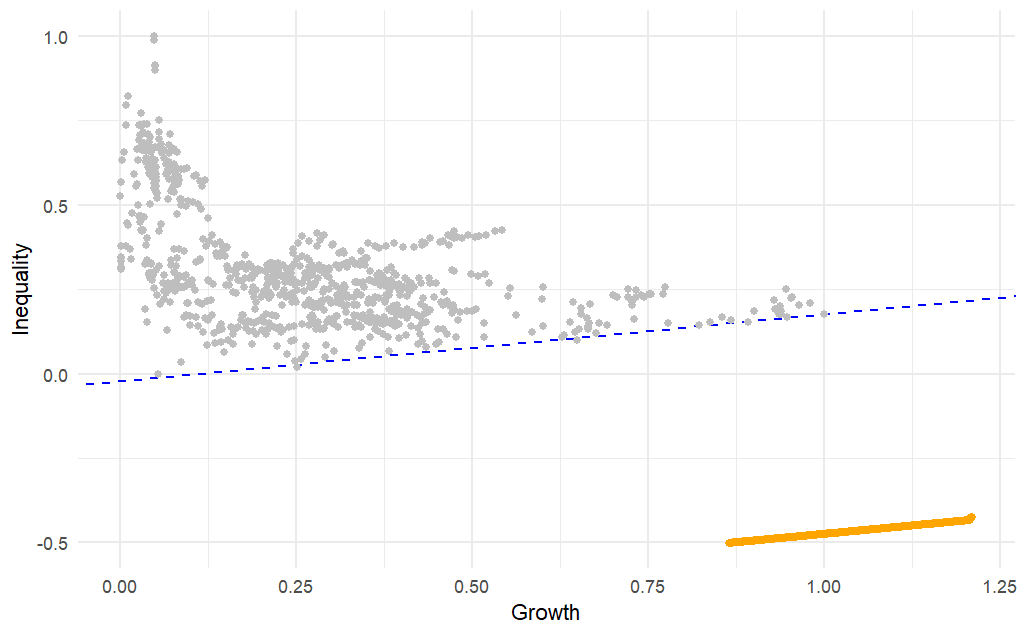
\includegraphics[width=0.8\textwidth]{trade_off.png}
    \caption{Trade-off between growth and inequality choices}
    \captionsetup{font=footnotesize}
    \caption*{\textbf{Notes:} The grey dots represent the scatter plot between (normalised) growth and inequality (in observed values). The lower blue line shows the Pareto-optimal solution, while the higher blue line is derived from the Pareto-optimal solution with an added penalty for inequality. This penalty can be interpreted as non-economic factors (such as fairness) influencing the inequality choice. The higher blue line reflects the inequality choices of developed countries around the world.}
    \label{fig:trade_off}
\end{figure}

Figure \ref{fig:trade_off} illustrates the relationship between normalised growth and inequality, highlighting the trade-offs between these two variables. The grey scatter points represent observed data, capturing the covariation of growth and inequality across different scenarios or regions. The wide dispersion of these points indicates significant variability in the interaction between growth and inequality. The lower blue line represents the Pareto-optimal frontier, which delineates the most efficient trade-offs between the two variables. Any point on this frontier reflects an optimal scenario in which it is impossible to increase growth without exacerbating inequality or reduce inequality without compromising growth. This frontier serves as the baseline for purely economic optimisation. In its original scale, the Pareto-optimal frontier corresponds to growth values ranging from approximately 38,031 to 164,510 and inequality values ranging from 12.58 to 26.73. 

Interestingly, the growth-inequality relationship observed in developed countries appears to run parallel to the Pareto-optimal frontier, suggesting a similar slope. To reflect this observed pattern, an upper blue line is plotted, representing the Pareto optimal frontier adjusted for an inequality penalty. This penalty may account for noneconomic factors, such as societal preferences for fairness or equity, which may influence policy decisions. Importantly, while the Pareto-optimal frontier is derived purely from economic choices, the gap between the two blue lines (the penalty) is hypothesised to reflect the influence of these non-economic factors. The analysis indicates that if inequality were solely an economic choice, its levels would likely be lower than observed due to the absence of noneconomic penalties. However, even when noneconomic factors are accounted for, the trade-off between growth and inequality remains evident, albeit within controlled limits. To further quantify this trade-off, a regression analysis was conducted between normalised growth and inequality. 

The regression results reveal a significant positive relationship, with a coefficient of \(0.241\) (\(p < 0.01\)), suggesting that a higher normalised GDP per capita is associated with a higher normalised inequality. The model explains \(85.2\%\) of the variance in inequality (\(R^2 = 0.852\)) and demonstrates a strong fit, as indicated by an adjusted \(R^2\) of \(0.850\). The \(F\)-statistic of \(563.175\) (\(p < 0.01\)) confirms the overall significance of the model, while the residual standard error of \(0.033\) suggests relatively low prediction errors, underscoring the robustness of the analysis. In conclusion, the findings highlight that even when societies have the ability to choose optimal levels of inequality, increased inequality may still be tolerated to some extent, provided it remains within controlled boundaries. This underscores the persistent trade-off between growth and inequality, influenced by both economic and noneconomic factors.


\section{If technology is beyond a tool} \label{sec:technology}

Inequality has multiple causes, including economic, social, and political factors. Thomas Piketty \parencite*{piketty2014capital} argues that the rise in inequality in the developed world is primarily due to the higher return on capital compared to economic growth, leading to wealth accumulation by the already wealthy. Economists Christoph Lakner and Branko Milanovic, through the Elephant curve \parencite*{lakner2016global}, suggest that globalisation has benefited the global superrich and emerging middle classes while harming the poor and middle class in developed countries. The Skill-biased Technical Change theory \parencite{acemoglu2002technical} links technological progress, driven by globalisation, to rising social division. However, sociologists argue that technological development alone does not increase inequality; it must also be influenced by sociopolitical factors such as labour market patterns \parencite{morris1999inequality,neckerman2007inequality}. Technological unemployment and job polarisation are current issues in the labour market \parencite{spencer2018fear,fernandez2012job}. Political scientists also highlight institutions, particularly property rights and labour market regulations, as key drivers of inequality \parencite{boix2010origins}.

Although the factors that contribute to inequality are well understood, the role of technology in exacerbating inequality remains unclear. From an economic point of view, technology causes conditionally inequality in the race between education and technology \parencite{card2002skill}. From a socio-political perspective, technology causes inequality conditionally on the race between institutions and technology \parencite{kristal2017causes}. However, both perspectives ultimately support the view that technology conditionally contributes to inequality, similar to technology experts\footnote{Vogels, E. A., Rainie, L., \& Anderson, J. (2020, June 30). \textit{Tech is just a tool}. Pew Research Center. Retrieved November 19, 2024, from \href{https://www.pewresearch.org/internet/2020/06/30/tech-is-just-a-tool/}{https://www.pewresearch.org/internet/2020/06/30/tech-is-just-a-tool/} } arguing that `technology is just a tool,' and the resulting inequalities stem from human choices (such as those shaped by education and institutions). However, the question of whether technology is value neutral has been raised by \textcite{miller2021technology}. In contrast to the slogan `guns don’t kill, people kill,' \textcite{kroes2008morality} writes:

\begin{quote}
A gun is not a mere instrument, a medium for the free will of human beings; it helps to define situations and agents by offering specific possibilities for action.
\end{quote}

Clearly, each technological artefact is created with a specific purpose which defines its essence. Technology can be defined as the application of scientific knowledge, tools and techniques to solve problems, improve processes, and create products that address particular needs \parencite{arthur2009nature}. However, a technological object does not arise spontaneously; it is the product of accumulated knowledge and experience. For a tech object to evolve into an innovation with broader societal and economic impacts, it must interact within a network system, generating spillover effects. In this context, inequality can be unconditionally driven by the technology network itself. This study emphasises that the nature of technological development is inseparable from a network system. In \textit{The Question Concerning Technology}, \textcite{heidegger2009question} posits that technology is not merely a collection of tools, but a mode of revealing a way in which humans come to understand and interact with the world. Drawing on the actor-network theory of \textcite{latour2007reassembling}, the essence of technology lies in its ability to connect and influence other entities, distributing the agency across the network rather than centring it solely on human intention. Leaving traditional philosophical approaches, this study employs the simulation of a technological network to investigate the following question.
\begin{quote}
    Q2: If technology is beyond a tool, does it unconditionally cause inequality?
\end{quote}
Here, `beyond a tool' refers to defining technology not merely as a process or a product but as the dynamic interaction between these elements within a network. Thus, the concept of technology in this study closely aligns with that of innovation. Establishing this definition is crucial, as it directly relates to the term `unconditionally' in the research question. The term `unconditionally' is understood to mean being independent of human choices, such as education or institutional frameworks, which might otherwise condition whether technology causes inequality. In other words, this study emphasises the role of the network as the essence of technology, proposing that it causes inequality irrespective of human decisions. One might argue that a network is no different from a society, but I contend that it is not a matter of choice; rather, it operates as a law.

\subsection{Data and methods}
To explore this question, I simulate the wealth accumulation dynamics of agents over time, incorporating various parameters to capture the evolving nature of wealth and technology adoption. These parameters include the number of agents \(n\), the number of time periods \(T\), and the elasticities of capital \(\alpha\) and labour \(\beta\) in the wealth function, with the constraint that \(\alpha + \beta = 1\). Other key parameters include the capital accumulation rate \(r\), the base probability of technology adoption \(p\), the growth factor for technology adopters \(m\), the probability of initial connection between agents \(d\), the boost from mutual learning \(b\), and the probability of new connections when agents share common friends \(q\).

\begin{itemize}
    \item The initial wealth of each agent, \(W_i(0)\), is determined by a Cobb-Douglas production function, which incorporates the agent's initial level of technology \(T_i(0)\), capital \(K_i(0)\), and labour \(L_i(0)\). The wealth is updated for each period using the same functional form, where \(W_i(t) = T_i(t) \cdot K_i(t)^\alpha \cdot L_i(t)^\beta\), with \(t\) representing the current period of time. The capital of each agent is updated based on their accumulated wealth, using the formula \(K_i(t) = K_i(t-1) + r \cdot W_i(t)\).
    \item Technology adoption occurs through two mechanisms: independent adoption, where each agent has a base probability \(p\) of adopting technology, and network influence, where the probability of adoption increases with the number of adopting neighbours. The adoption probability \(P_{\text{adopt}, i}\) for agent \(i\) is given by \(P_{\text{adopt}, i} = 1 - (1 - 0.05)^{N_{\text{adopt}, i}}\), where \(N_{\text{adopt}, i}\) represents the number of adoptive neighbours. When both agents in a connection have adopted technology, their productivity increases, as indicated by \(T_i(t) = T_i(t) \cdot b^{N_{\text{adopt}, i}}\).
    \item Additionally, agents may form new connections if they share common friends, with a probability \(q\) given by: If \(|C_{ij}| > 0\), then \(P_{\text{connect}} = q\), where \(C_{ij}\) is the set of common friends between agents \(i\) and \(j\). The Gini coefficient \(G\) is used to assess inequality within the wealth distribution in each time period, calculated using the formula \(G = \frac{1}{2 \mu n^2} \sum_{i=1}^n \sum_{j=1}^n |W_i - W_j|\), where \(W_i\) represents the wealth of agent \(i\), \(\mu\) is the mean wealth and \(n\) is the total number of agents. This Gini coefficient provides a measure of wealth inequality that reflects the cumulative effects of wealth accumulation, technology adoption, and network dynamics.
\end{itemize}

The simulation involves a system of 100 agents that interact over 30 time periods. Agents accumulate wealth through three main factors: capital, labour, and technology. Capital contributes 30\% to wealth generation, while labour contributes 70\%, reflecting the elasticities of capital and labour in the wealth function. In addition, technology plays a critical role in boosting agents' wealth. Each agent has an initial chance of adopting technology and, once adopted, technology increases their productivity by 20\%. Agents also interact within a social network, where there is a probability 10\% of initial connection between them. These network connections enable agents to engage in mutual learning, further boosting their wealth by 5\%. Furthermore, if agents share common connections, there is a 5\% chance of forming new ties, simulating triadic closure within the network.

Each agent starts with randomly varied endowments: capital is normally distributed with a mean of 50 and a standard deviation of 10, labour with a mean of 1 and a standard deviation of 0.2, and technology adoption with a mean of 1 and a standard deviation of 0.3. Initially, no agents have adopted technology and their wealth is set to zero. Over time, agents' wealth, capital, and technology levels evolve on the basis of their personal endowments, interactions with others, and technology adoption. The network structure and mutual learning effects help to amplify the wealth accumulation of agents, facilitating the diffusion of technology, and improving overall productivity (see the algorithm in Appendix \ref{ap:simulation}).

\subsection{Results and discussion}
\begin{figure}[H]
    \centering
    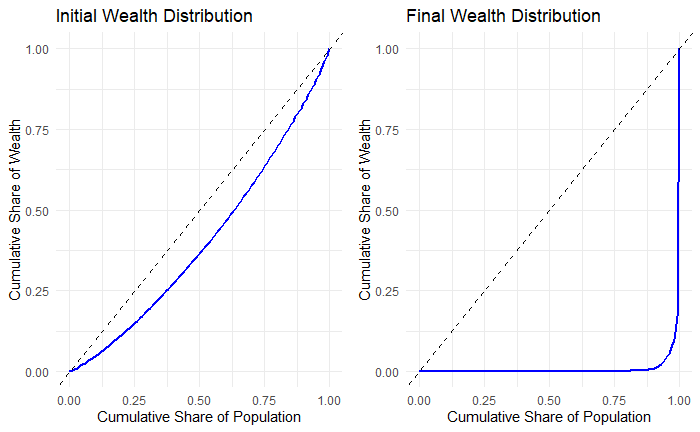
\includegraphics[width=0.7\textwidth]{wealth_dist.png}
    \caption{Wealth distribution over time}
    \label{fig:wealth_dist}
\end{figure}

Figure \ref{fig:wealth_dist} presents Lorenz curves depicting wealth distribution in a population at two time points. The left panel shows the initial wealth distribution, while the right panel illustrates the final wealth distribution after a simulated period of wealth accumulation and economic interaction. Initially, the Lorenz curve is moderately curved and close to the 45-degree line of perfect equality, indicating a relatively even distribution of wealth with only moderate inequality. The slight deviation suggests that most of the population has a proportionate share of wealth. In contrast, the final distribution exhibits a highly skewed Lorenz curve that deviates significantly from the equality line. The curve remains nearly flat for the majority of the population, indicating negligible cumulative wealth, and rises steeply near the end, where a small fraction of the population holds nearly all the wealth. This dramatic change highlights the emergence of extreme inequality, with wealth concentrated in the hands of a small elite. The comparison of the two panels reveals how wealth inequality intensifies over time. Initially equitable, the system evolves through mechanisms like capital accumulation, network effects, and technological advantages, leading to extreme wealth concentration. This pattern reflects the `Matthew Effect,' where initial advantages compound over time, marginalising less-advantaged individuals.


\begin{figure}[H]
    \centering
    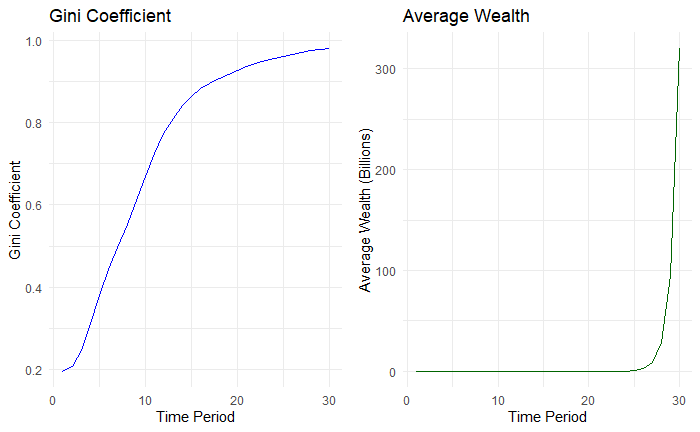
\includegraphics[width=0.7\textwidth]{gini_wealth.png}
    \caption{Inequality and Growth over time}
    \label{fig:gini_wealth}
\end{figure}

Figure \ref{fig:gini_wealth} illustrates the dynamics of wealth inequality and accumulation over time, using two distinct plots. The left plot tracks the Gini coefficient, a measure of inequality, which starts at a moderate level near 0.2 and steadily increases over 30 time periods, approaching a value of 1. This trend suggests that wealth becomes increasingly concentrated among a small subset of agents as time progresses. The sharp increase in the Gini coefficient highlights the accelerating inequality, potentially driven by mechanisms such as network effects or selective technology adoption that favour certain individuals over others. The right plot displays the average wealth of agents, measured in billions. Initially, average wealth remains nearly stagnant, indicating slow accumulation during the early time periods. However, a dramatic exponential increase occurs toward the end of the time frame. This rapid growth likely reflects the compounding effects of technology adoption and capital accumulation, where wealthier or more technologically advanced agents benefit disproportionately. 

Together, the two plots reveal a strong interplay between wealth growth and inequality. Although average wealth grows exponentially, the corresponding rise in the Gini coefficient indicates that gains are unevenly distributed, with only a few agents reaping the majority of benefits. This pattern could be explained by feedback mechanisms, such as preferential attachment in networks, where agents with initial advantages, such as higher connectivity or early technology adoption, consolidate wealth more effectively over time. The findings underscore the potential for technology and network effects to exacerbate inequality, suggesting a need for policy interventions to ensure that the benefits of economic growth and technological progress are more equitably distributed.

\section{Conclusion} 
This study brings to light two fundamental questions about the nature of development: whether inequality is an economic choice and whether technology inherently causes inequality. These inquiries highlight the complex trade-offs and dynamics shaping economic growth and societal equity.
\begin{itemize}
    \item First, the analysis underscores that inequality is not merely a by-product of economic systems but a result of deliberate choices made in policy and governance. Although extreme inequality hinders sustainable growth, controlled levels of inequality can coexist with or even support growth under certain conditions. This raises the critical question of priorities: Should policymakers focus on reducing inequality, even at the expense of growth, or strike a balance that allows moderate inequality for the sake of fostering competition and innovation?
    \item Second, the study challenges the notion of technology as a neutral tool, revealing how its structural dynamics and network effects inherently exacerbate inequality. Simulations show that the diffusion and impact of technology often amplify initial disparities, leading to a concentration of wealth and opportunities. This finding poses a crucial problem: even if technology is not inherently biased,  integration into existing systems unconditionally drives inequality, regardless of human intentions or interventions.
\end{itemize}

Through multiobjective optimisation and simulations, this research reveals that inequality and technology are central to the development process, each requiring nuanced understanding and careful management. Policymakers must navigate these interdependencies, acknowledging that growth, equity, and technological progress are not independent phenomena, but deeply interconnected dimensions of development. By addressing these questions, the study highlights the urgent need for deliberate equity-focused strategies to harness growth and technology in ways that promote inclusive and sustainable development.

\newpage
\printbibliography

\newpage
\appendix
\small
\section{Non-dominated Sorting Genetic Algorithm II} \label{ap:NSGA}
\input{NSGA}
\newpage
\section{Wealth Inequality Simulation with Network Effects}
\label{ap:simulation}
\begin{algorithm}
\scriptsize
\caption{Wealth Inequality Simulation with Network Effects}
\begin{algorithmic}[1]
\Require Number of agents $n_{\text{agents}}$, number of periods $n_{\text{periods}}$, parameters $\alpha$, $\beta$, $r$, and network properties.
\State \textbf{Initialisation:}
\State Set random seed for reproducibility.
\State Initialise agents with:
\State \hspace{\algorithmicindent} \textbf{Capital:} $C_i \sim \mathcal{N}(50, 10)$
\State \hspace{\algorithmicindent} \textbf{Labour:} $L_i \sim \mathcal{N}(1, 0.2)$
\State \hspace{\algorithmicindent} \textbf{Technology:} $T_i \sim \mathcal{N}(1, 0.3)$
\State \hspace{\algorithmicindent} \textbf{Tech adoption status:} $A_i \gets \text{False}$
\State \hspace{\algorithmicindent} \textbf{Wealth:} $W_i \gets T_i \cdot (C_i^\alpha) \cdot (L_i^\beta)$
\State Generate a random network with connection probability $p$.

\For{$t = 1$ to $n_{\text{periods}}$}
    \State \textbf{Independent Technology Adoption:}
    \For{$i = 1$ to $n_{\text{agents}}$}
        \If{$\text{rand}() < \text{tech\_adoption\_rate}$}
            \State $A_i \gets \text{True}$
        \EndIf
    \EndFor

    \State \textbf{Technology Transfer within Network:}
    \For{$i = 1$ to $n_{\text{agents}}$}
        \If{$A_i = \text{False}$}
            \State Identify neighbours $\mathcal{N}(i)$.
            \State Calculate probability of adoption: $P_{\text{transfer}} = 1 - (1 - 0.05)^{|\mathcal{N}_A(i)|}$.
            \If{$\text{rand}() < P_{\text{transfer}}$}
                \State $A_i \gets \text{True}$
            \EndIf
        \EndIf
    \EndFor

    \State \textbf{Mutual Learning:}
    \For{$i = 1$ to $n_{\text{agents}}$}
        \If{$A_i = \text{True}$}
            \State Identify neighbours $\mathcal{N}_A(i)$ with $A_j = \text{True}$.
            \State Update technology: $T_i \gets T_i \cdot (\text{mutual\_learning\_boost})^{|\mathcal{N}_A(i)|}$
        \EndIf
    \EndFor

    \State \textbf{Triadic Closure:}
    \For{$i = 1$ to $n_{\text{agents}}$}
        \For{each $j$ such that $i \neq j$}
            \State Check for common neighbours $k$ between $i$ and $j$.
            \If{not connected and $\text{rand}() < \text{triadic\_closure\_prob}$}
                \State Add edge between $i$ and $j$.
            \EndIf
        \EndFor
    \EndFor

    \State \textbf{Update Wealth and Capital:}
    \For{$i = 1$ to $n_{\text{agents}}$}
        \State Update wealth: $W_i \gets T_i \cdot (C_i^\alpha) \cdot (L_i^\beta)$.
        \State Update capital: $C_i \gets C_i + r \cdot W_i$.
    \EndFor

    \State \textbf{Record Metrics:}
    \State Compute Gini coefficient: $\text{Gini}(W)$.
    \State Record average wealth: $\bar{W} = \frac{1}{n_{\text{agents}}} \sum_{i=1}^{n_{\text{agents}}} W_i$.
\EndFor
\end{algorithmic}
\end{algorithm}
\end{document}
